.n the screen.\section{Material \& Methods}
%What is possible in the system:
\subsection{Choice of device}
We aim to design a system that is capable of providing a multitude of interaction methods. The Hololens' persistent object showcase serves as example for the types of interaction users should be able to have within our system: virtual objects can be \textit{selected, placed, scaled} and \textit{rotated} freely in 3D space. Each interaction is either mapped to a specific hand gesture or performed using a touch screen.

Gestures are chosen to mimic real world interactions. The Hololens is a portable AR head-mounted display, offering the FOV of approximately 30 degrees. This device is capable of tracking user position in a room provided the system is properly set up. Interaction is facilitated by gaze visualised as a cursor and the hand-based gesture of tapping in mid-air. 

We also considered other devices for our system. Daqri offers another portable AR head-mounted display with the Daqri Smart Helmet (FOV of approximately 44 degrees). Its major drawback, however, is that the available interaction modalities do not support hand gesture detection, so interaction depends primarily on gaze and Bluetooth controllers. 

VR head-mounted displays are also an option when used in conjunction with additional hand tracking devices. While in an AR environment virtual objects need to be embedded in a real room, in a VR environment, such a room with added objects can be simulated. We decided that VR was a good choice for our project, because the virtual scene can be held constant and manipulated for a consistent experiment.

Of all the VR HMDs, we picked the HTC Vive which has a FOV of 110 degrees. In conjunction with a Leap Motion, it offers hand tracking that can be seamlessly integrated to facilitate gesture-based interaction. Furthermore, the Vive can be connected to a touch screen, such as a smartphone or tablet, for different interaction input modalities.
\subsection{Interaction methods}
As mentioned before, two interaction methods are to be implemented within the system: gesture-based and touch screen-based. Table~\ref{interactions} presents an overview of specific realisations of interactions. We have excluded scaling from the list of available manipulations, because early on during the project it was decided that scaling was inapplicable for our use case. However, the acts of selection/deselection, translation and rotation are enabled in our system.

\begin{table*}
\centering
\begin{tabular}{|l|p{5cm}|p{5cm}|}
\hline
\textbf{Interaction type} & \textbf{Gestures} & \textbf{Touch screen} \\
\hline
Selection & Gaze at object and use thumbs up & Gaze at object and tap \\
\hline
Deselection & Thumbs down & Double tap \\
\hline
Translation & Pinch with thumb and index finger and move the hand & Select virtual axis with a tap and swipe \\
\hline
Rotation & Both hands using the handle bar metaphor & Select virtual axis with a tap and rotate the touch screen device \\
\hline
\end{tabular}
\caption{Overview of interaction implementations in our project}
\label{interactions}
\end{table*}

Selection is accomplished by combining gaze and touch, as mentioned before, it is a common approach in virtual interactions. In our system, users can pre-select the desired object by looking at it and then use a gesture or perform an action via touch screen to confirm their selection. We decided that this combination of gaze/touch is convenient for users and reduces the probability of errors, compared to, e.g., gazing at the object for a long time. We do not use a dedicated eyetracker, because we decided that it would be enough to use the centre of the front camera perspective of the HTC Vive to simulate gaze tracking in our project. Therefore, the users have to position their head in a way, so that the desired object becomes the centre of their field of view in order for it to be pre-selected. In our opinion, however, it does not significantly breach the immersion of interaction, because intuitively, people tend to centre their vision on an object they want to attend to. This centre of vision is marked by the presense of a tiny crosshair in the virtual space. When this crosshair is "touching" an object, it changes its colour to yellow. If the highlighted object is the desired one, the user can confirm the selection, using either the thumbs up gesture or a tap on the touch screen, depending on the current interaction method. For gesture recognition using Leap Motion, a thumbs up gesture was picked. Other gestures were considered, too, e.g., the tap in the air, but its realisation was found ineffective and awkward for users. A thumbs up is a gesture that is often used to express approval in real life, has a very clear form and was chosen for these reasons. After the object has been selected, it changes its colour from yellow to purple.

We decided to make deselection an explicit act for convenience of users. They do not need to look at the object once it has been selected to avoid unnecessary exhaustion. Neither is gaze required for deselection. So, after the user is done interacting with the object, they can deselect it using a thumbs down gesture or tap twice on the screen depending on the current interaction technique. The thumbs down gesture was chosen as a natural counterpart to the thumbs up gesture used for selection. However, it is more difficult to perform, so we decided to ease the detection of this gesture, so that users do not need their thumb showing strictly 90 degrees down. For the touch screen condition, we chose a double tap for deselection in order to make it a distinct action from selection and also less error-prone. We decided that accidental deselection might be more annoying for users than accidental selection, because they might be in the middle of some manipulation that would get aborted by an accidental single tap.

Speaking of manipulations, the way we implemented translation in our two conditions is very different. For Leap Motion, the user has to make a pinch gesture with their thumb and index finger and hold this gesture while they are moving their hand in the direction they want to move the selected object. Translation occurs in 3D space, where hand movements are tracked and the difference in coordinates in all directions is directly translated to the selected object. The user can perform the pinch anywhere in the space, so while moving their hand, they might get out of tracking range. If that happens, they should release the pinch, move their hand in the field of view of the Leap Motion sensors and perform the pinch gesture again. 

When using the touch screen, however, such direct translation in 3D is impossible, because the screen is only a 2D plane. We decided to solve this problem by forcing the user to move the object in this condition axis by axis. Once the object is selected, three axes appear at its centre, depicted by arrows: up-and-down, back-and-forth, left-and-right. Using the same gaze/touch selection technique as used for regular virtual objects, the user can select a desired arrow and perform a swiping movement on the screen. The screen needs to always be in landscape orientation and the swipe should be made from top to bottom.
The coordinates of the swipe are translated to the object along the selected axis with a fixed scale factor.
The scale factor arises from the fact that a difference of 1 pixel along the swipe of the touch input relates to a shift of 1 unit in the vr-scene.
Experimenting with this relation resulted in an seemingly appropriate factor of $1:1000$.
When the user wants to translate the object along another axis, they can just select a different arrow, no deselection of the current arrow is necessary, because this action is only applicable to virtual objects. In both conditions, as soon as the desired position of the target object is achieved, the object can be deselected using the applicable technique.

Implementing rotation was more difficult than implementing translation. At first, we thought that it is most intuitive to imagine a real object as a proxy for the target virtual object. As the user rotates this proxy, the rotation applied is directly translated onto the virtual object. Such an object in the gesture-based condition would be the user's hand and in the touch screen-based condition - the phone itself. However, we encountered a big problem when trying to implement this approach. When the user initiates rotation, the coordinate systems of the proxy and the target are forced to align, so that direct translation of the rotation coordinates is possible. This causes the target object to immediately change its orientation in space. Additionally, due to hand tracking of the Leap Motion, the release of the fist marking the end of rotation cannot be pinpointed in time precisely, so the target object gets rotated a bit after the user actually stops the manipulation. This behaviour is undesired, so we looked for a different approach. \cite{song2012} addresses the limitations of hand tracking with respect to rotation and proposes a handle bar metaphor. In our implementation, an invisible handle bar is pierced through the centre of the object. The user can remotely grab this bar by closing two fists and then keep them closed as they rotate the bar in 3D space. The rotation applied is then translated directly to the target object's bar. The process looks similar to what is depicted in figure~\ref{handle}.

\begin{figure}
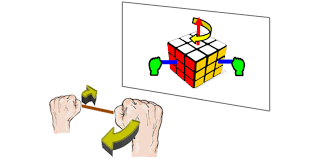
\includegraphics[width=0.48\textwidth]{handlebar}
\caption{
\textsf{Bimanual CLOSE fist gestures for rotating an object~\cite[p.~1302]{song2012}}
}
\label{handle}
\end{figure}

Rotation in the touch screen condition is implemented in a similar fashion to translation, axis by axis. The user can select the desired axis, as described before and then initiate rotation around this axis by holding the phone in the landscape orientation and pressing and holding two thumbs on the screen. While holding, the user can then rotate the phone back and forth and these rotation coordinates are then directly translated to the target object. If the user desires to rotate the object around another axis, they have to let go of the screen to stop the previous rotation and select the next axis by gazing at it and tapping on the screen.
\subsection{Implementation}

We worked with Unity version 5.4.0f during our project. It lets one easily integrate both the Leap Motion and an Android-based touch screen device. We used Unity Core Assets for Leap Motion version 3.0.0 and the Android SDK Tools version 25.2.3. Two Unity projects were created, one for each interaction method. Scripts were written in both C{\#} and Java Script languages.

In order for virtual objects to be selected, a layer called "Selectable" was created. The objects that are assigned to this layer can be manipulated by the user. In the Leap Motion condition manipulation occurs via gestures that are recognised by various custom-defined detectors. For instance, in order to detect a thumbs up gesture, we used the "and" combination of the "Extended Finger Detector" that defines that the thumb must be extended, while other fingers are not and the "Finger Direction Detector" that defines that the thumb must be extended in the upward direction with an acceptable level of tolerance for the inaccuracy of the user's gesture. Similarly, we used the "Pinch Detector" for the pinch gesture and the "Extended Finger Detector" that defines that all fingers must not be extended for fist recognition. Scripts can be assigned to detectors, they specify the actions to be performed once the gesture is recognised. In the touch screen condition, an additional layer was added for selection of axes that enable the user to manipulate objects. We called this layer "SelectableAxis".

The scene for our experimental use case which will be described in the next section was also designed in Unity.

\iffalse
While using our hands directly on objects to interact with them seems like an intuitive approach it is a very novel type of interaction in the context of human machine interfaces.
Interactions with technical systems has become an every day task in many peoples lives.
Using smartphones and tablets more often relies on touch surface interfaces even than on using a mechanical interface like a keyboard.

And exactly these two modes of interaction we aim to compare in our experiment:
The seemingly intuitive but novel hand gesture recognition vs. touch surface gesture recognition people are already familiar with from everyday use of smart phones.

Should contain:
	[X] What is possible in the system? (Martin)
        [X] Interaction with objects in 3d space X
        [X] Translation/Rotation/Scaling
	
    What the systems should be capable of? (Martin)
    	Intuitive input modality
        [ ] Gesture based interactions
        [ ] Tracking of user movements
    
     [ ] Why did we choose Leap/Touch Surfaces? (Thandi)
    	[ ] Touch Surfaces:
        	People are used to it (Smart Phones, Tablets etc.)
    	[ ] Leap:
        	Affordable
            Capable
            Customizable    
            
    [ ] Interaction methods
    	[ ] Overview in a table
        [ ] Explain choice of specific gestures
	
    Software Structure
      
	[X] Separate section - Experimental Design: (Martin)
		[X] Motivation
        [X] Scene Layout
    	[X] User Tasks
        [X] What was measured?
        [X] What was tested for?
    
    
Put the following on the appendix:
Why did we choose Unity? (Thandi)
    	*Documentation is good
        *Has all interfaces to easily integrate our devices
    
    System specifics:
    	*Which modules (Version numbers)
        *What programming language
     
\fi